\begin{figure}
    \centering
    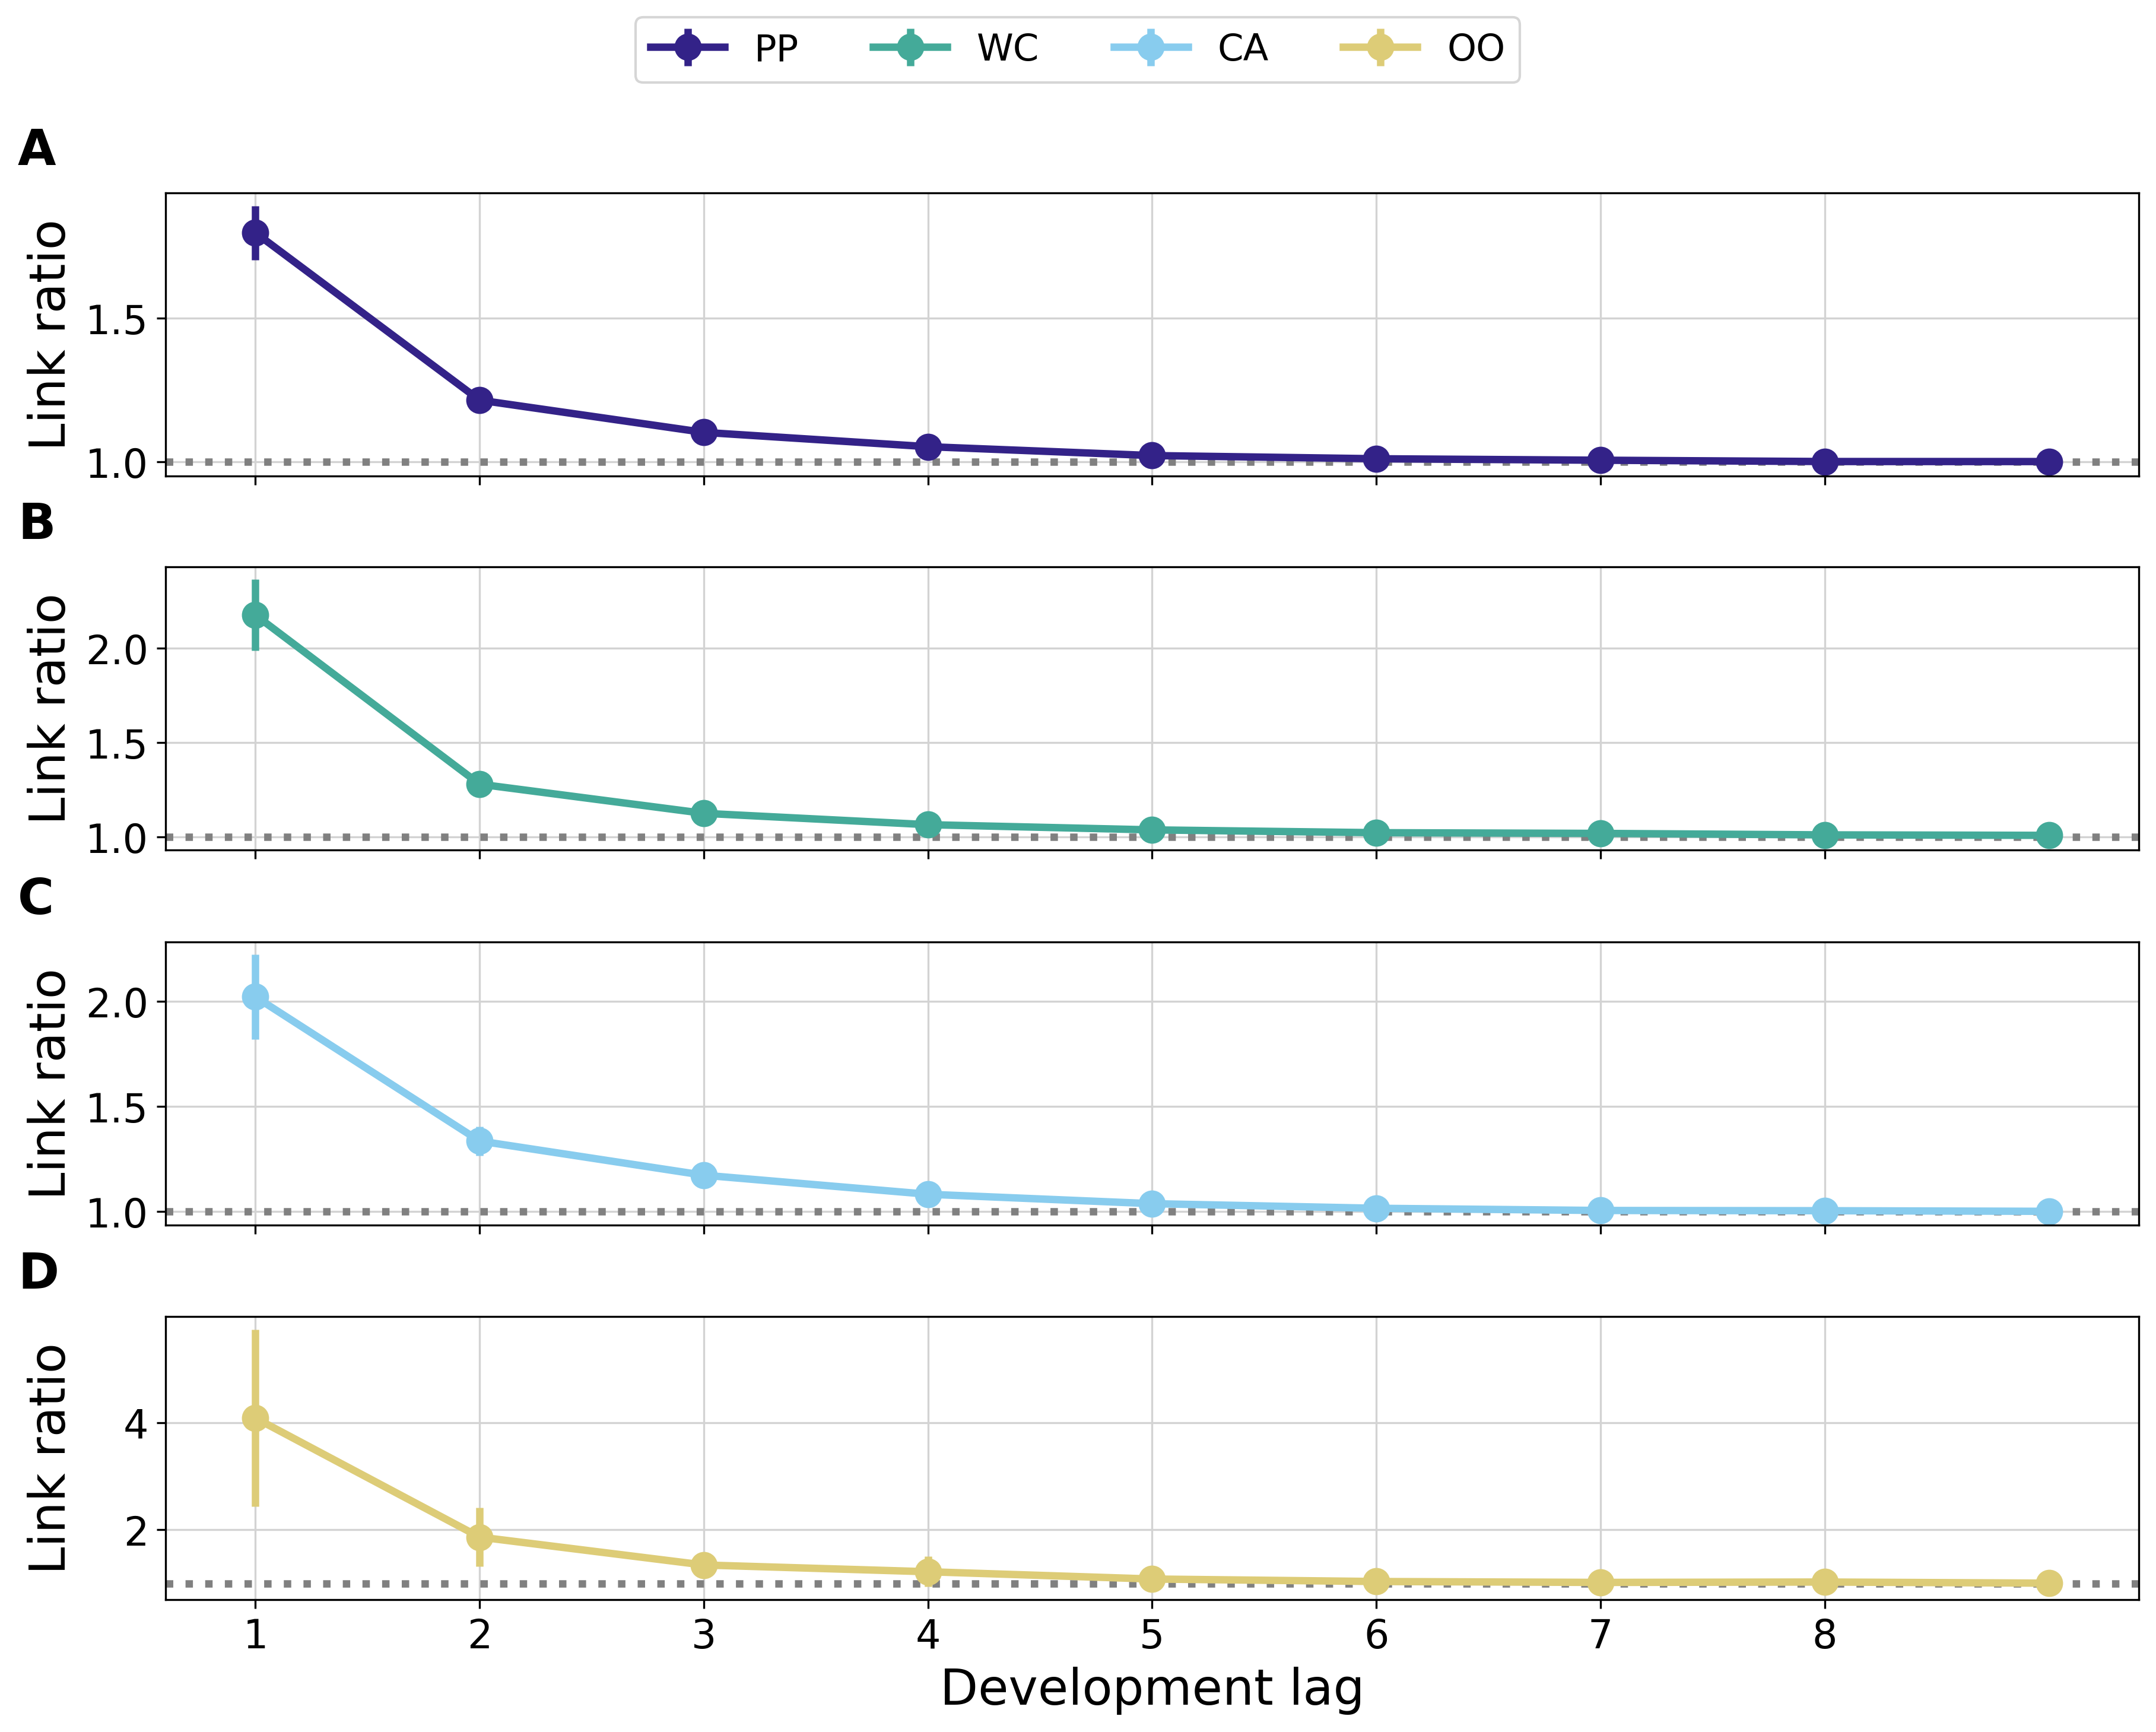
\includegraphics[scale=0.5]{\figures/atas.png}
    \caption{
        The empirical link ratios by line of business in
        the \cite{meyers2015} dataset.
        Points indicate the mean across triangles,
        and vertical line segments show 2 standard
        deviations.
    }
\end{figure}

\begin{figure}
    \centering
    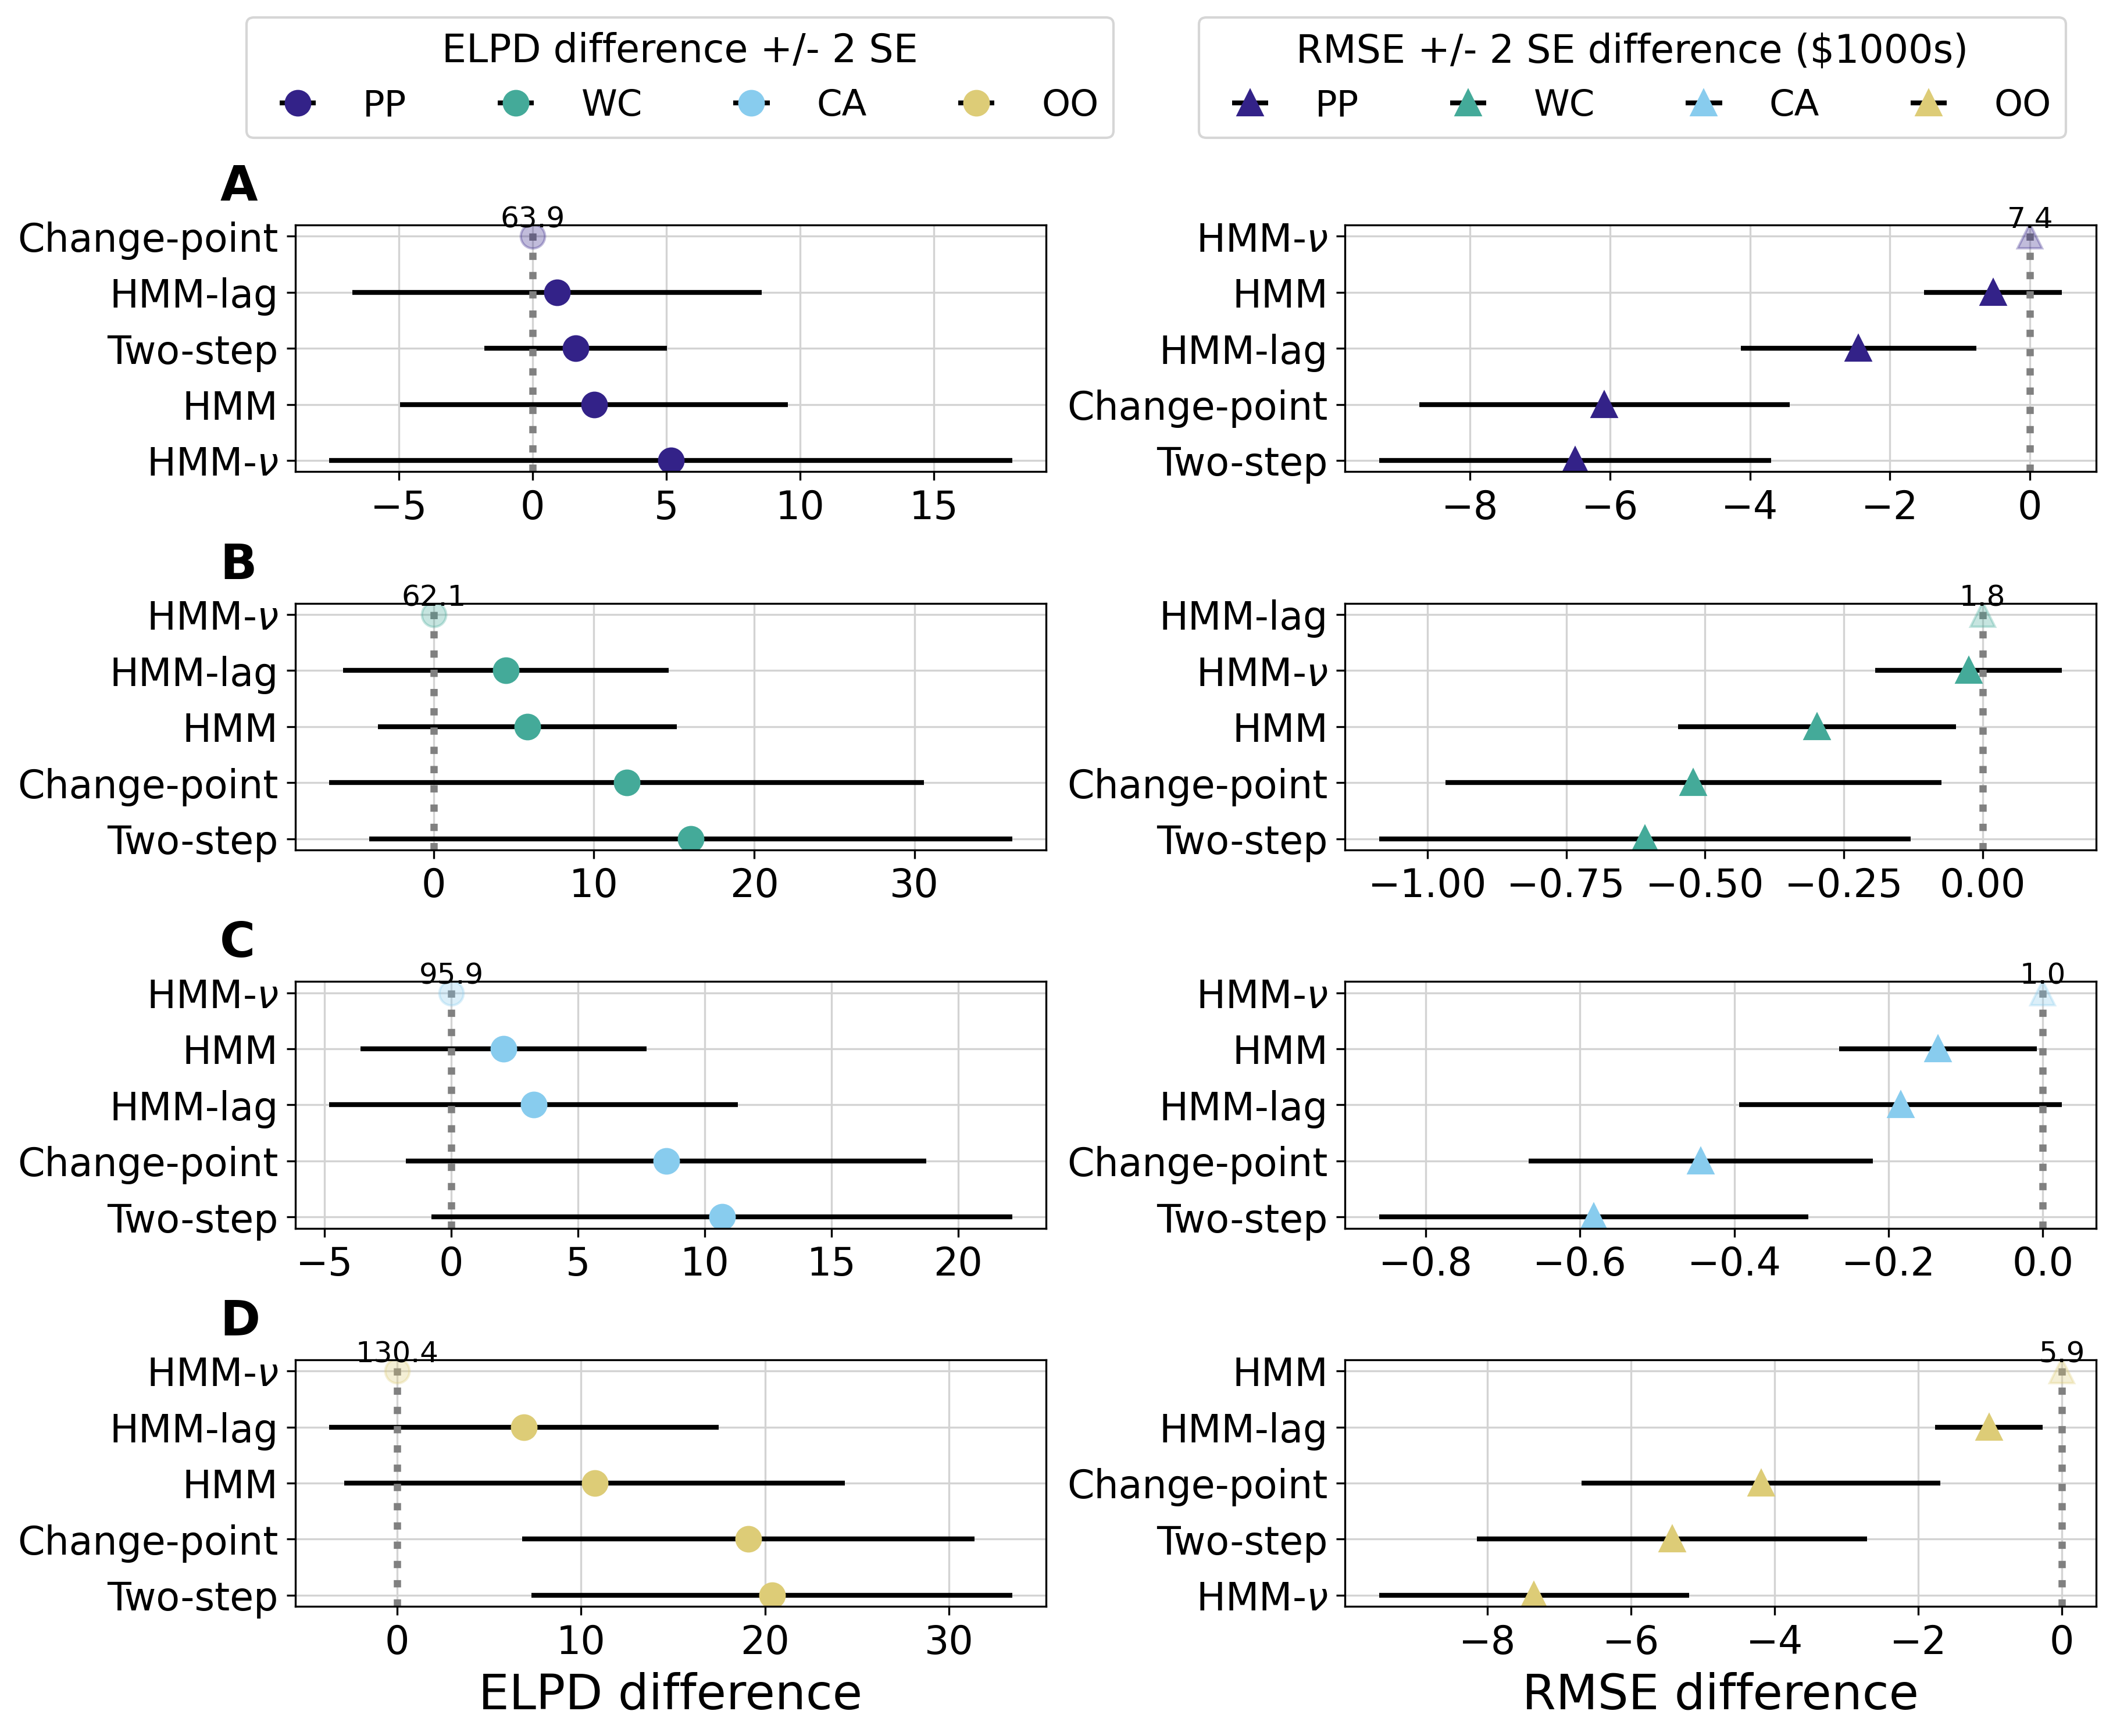
\includegraphics[scale=0.5]{\figures/scores.png}
    \caption{
        The ELPD (left column) and RMSE (in dollars; right column)
        for each of the four models and line of business
        in the industry backtest. The ELPD values are remove
		any cell's predictions that have a log likelihood value
		$\leq -100$, to not bias the results unfairly towards poorly
		performing predictions.
    }
\end{figure}


\begin{figure}
    \centering
    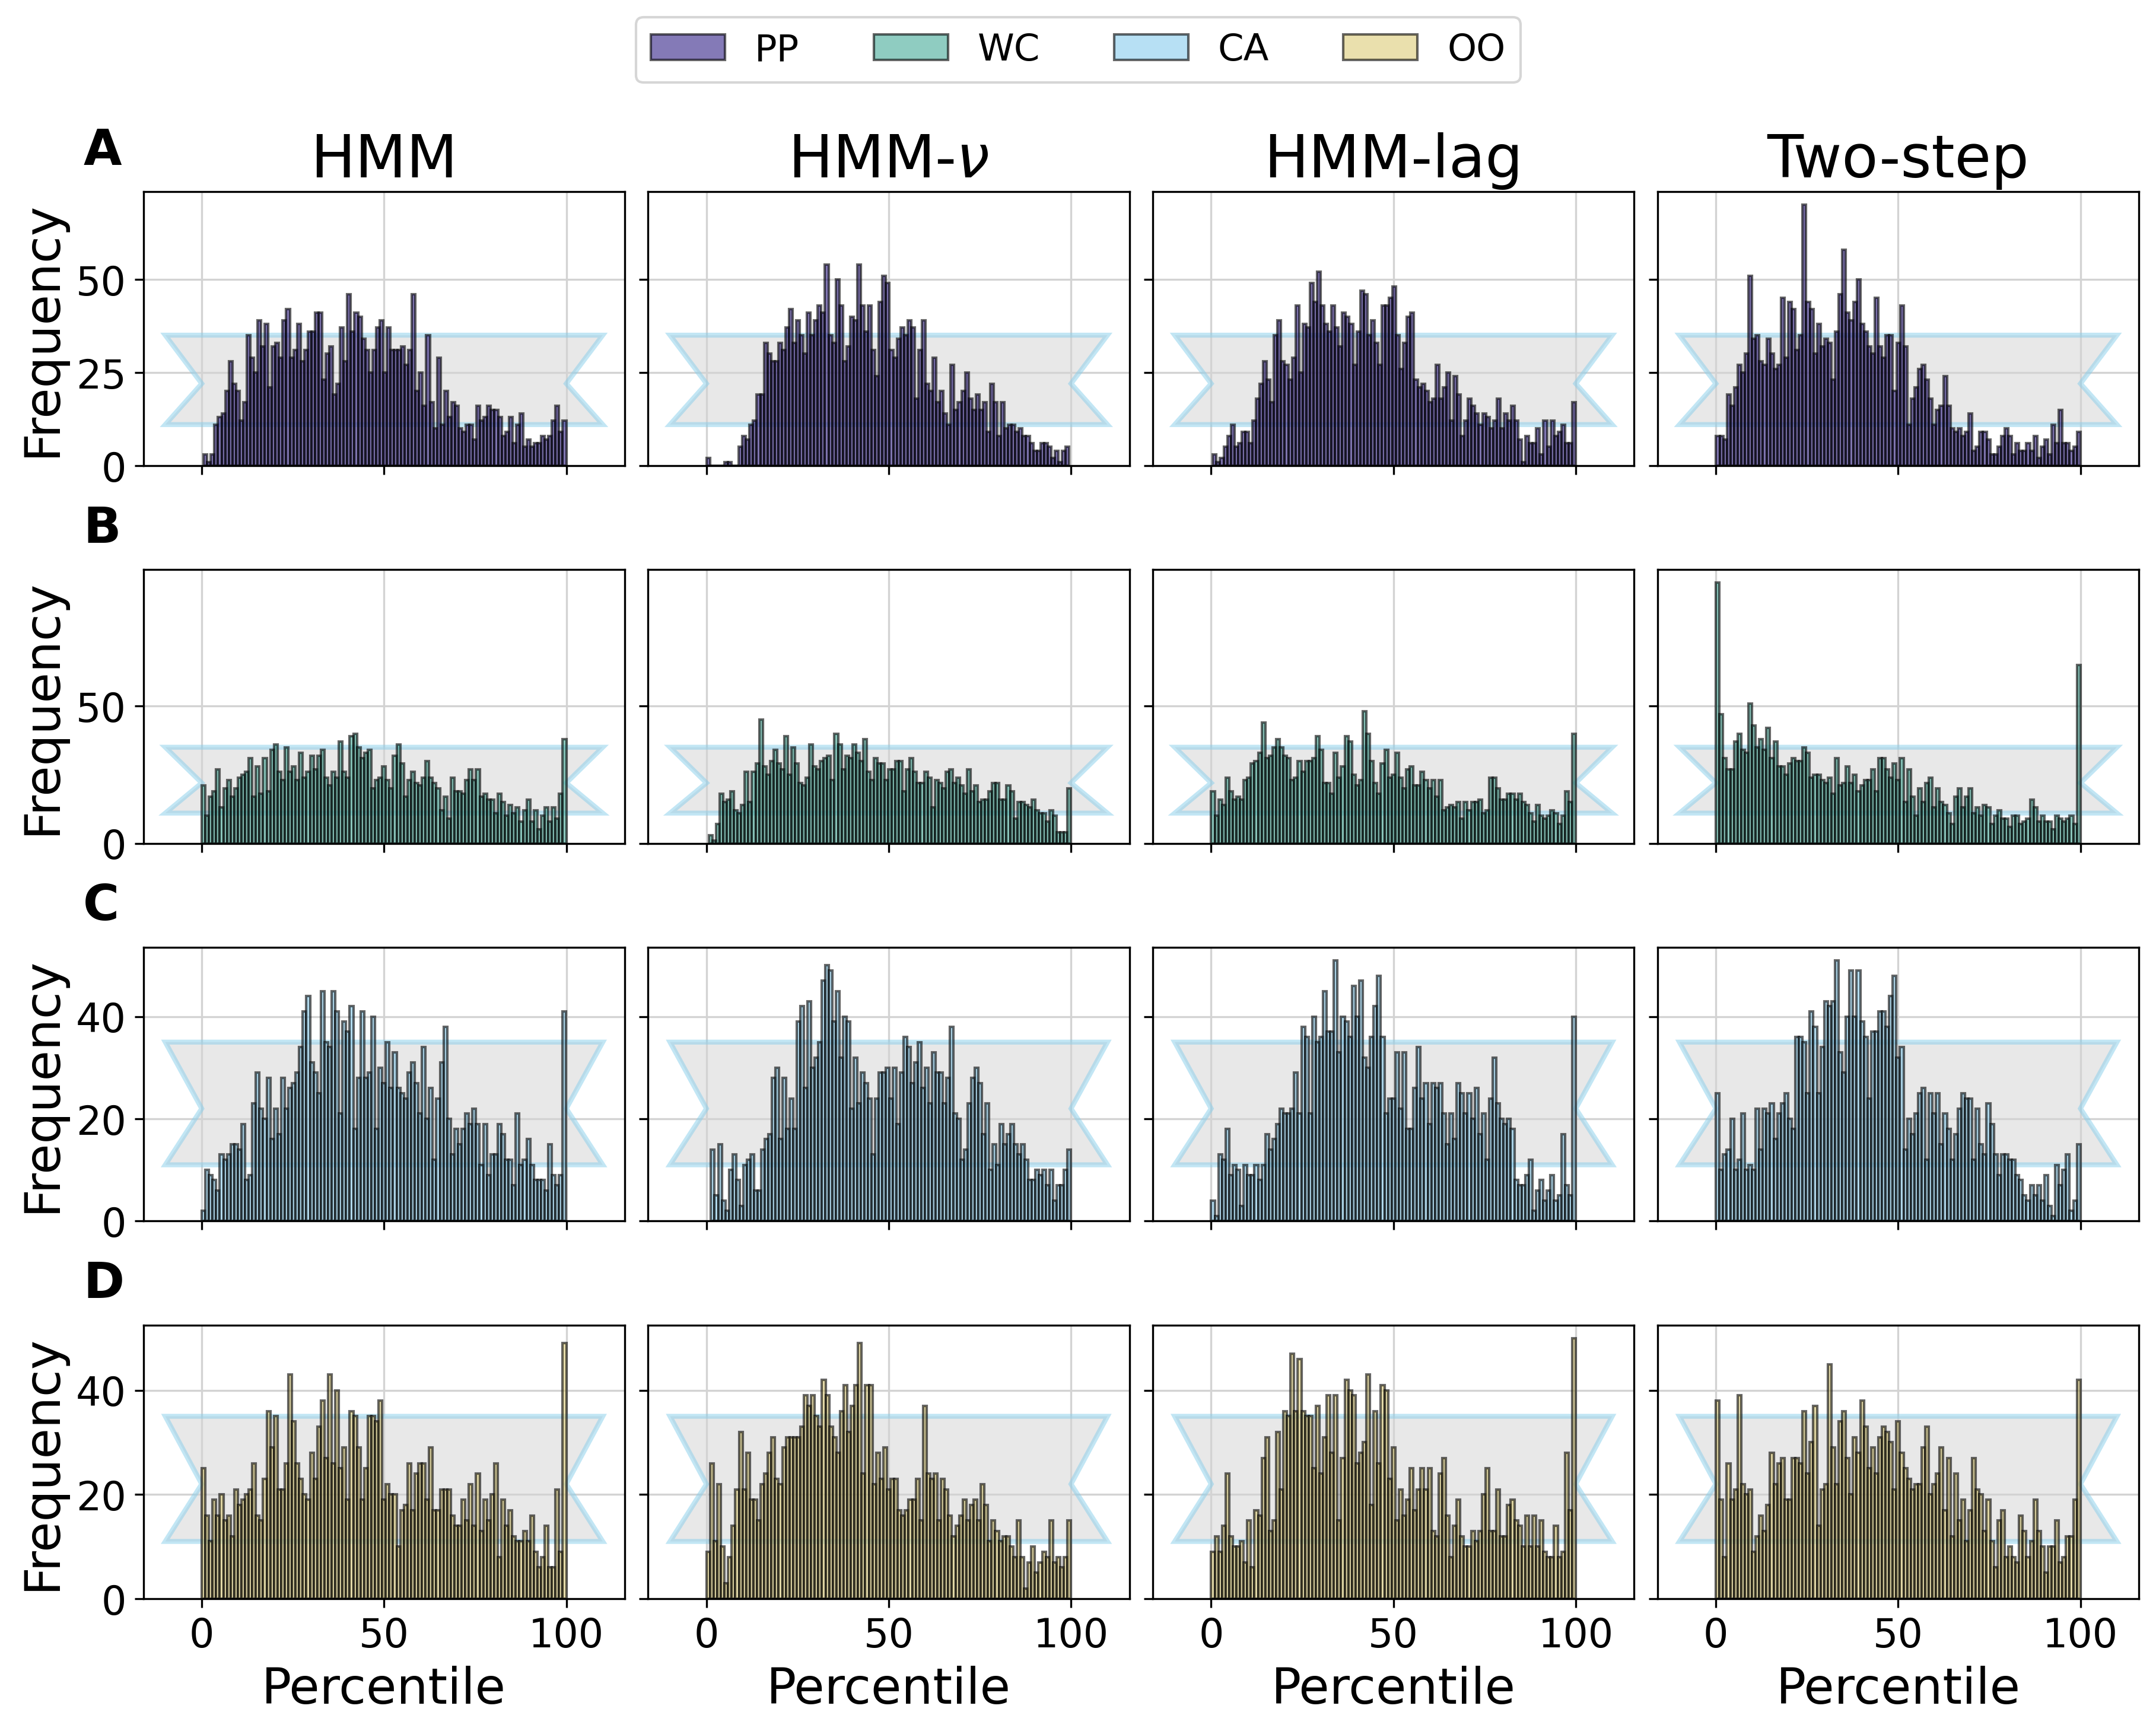
\includegraphics[scale=0.5]{\figures/calibration.png}
    \caption{
        Percentiles of the true values on the posterior distributions
        for each model and line of business in the backtest.
    }
\end{figure}

\begin{figure}
    \centering
    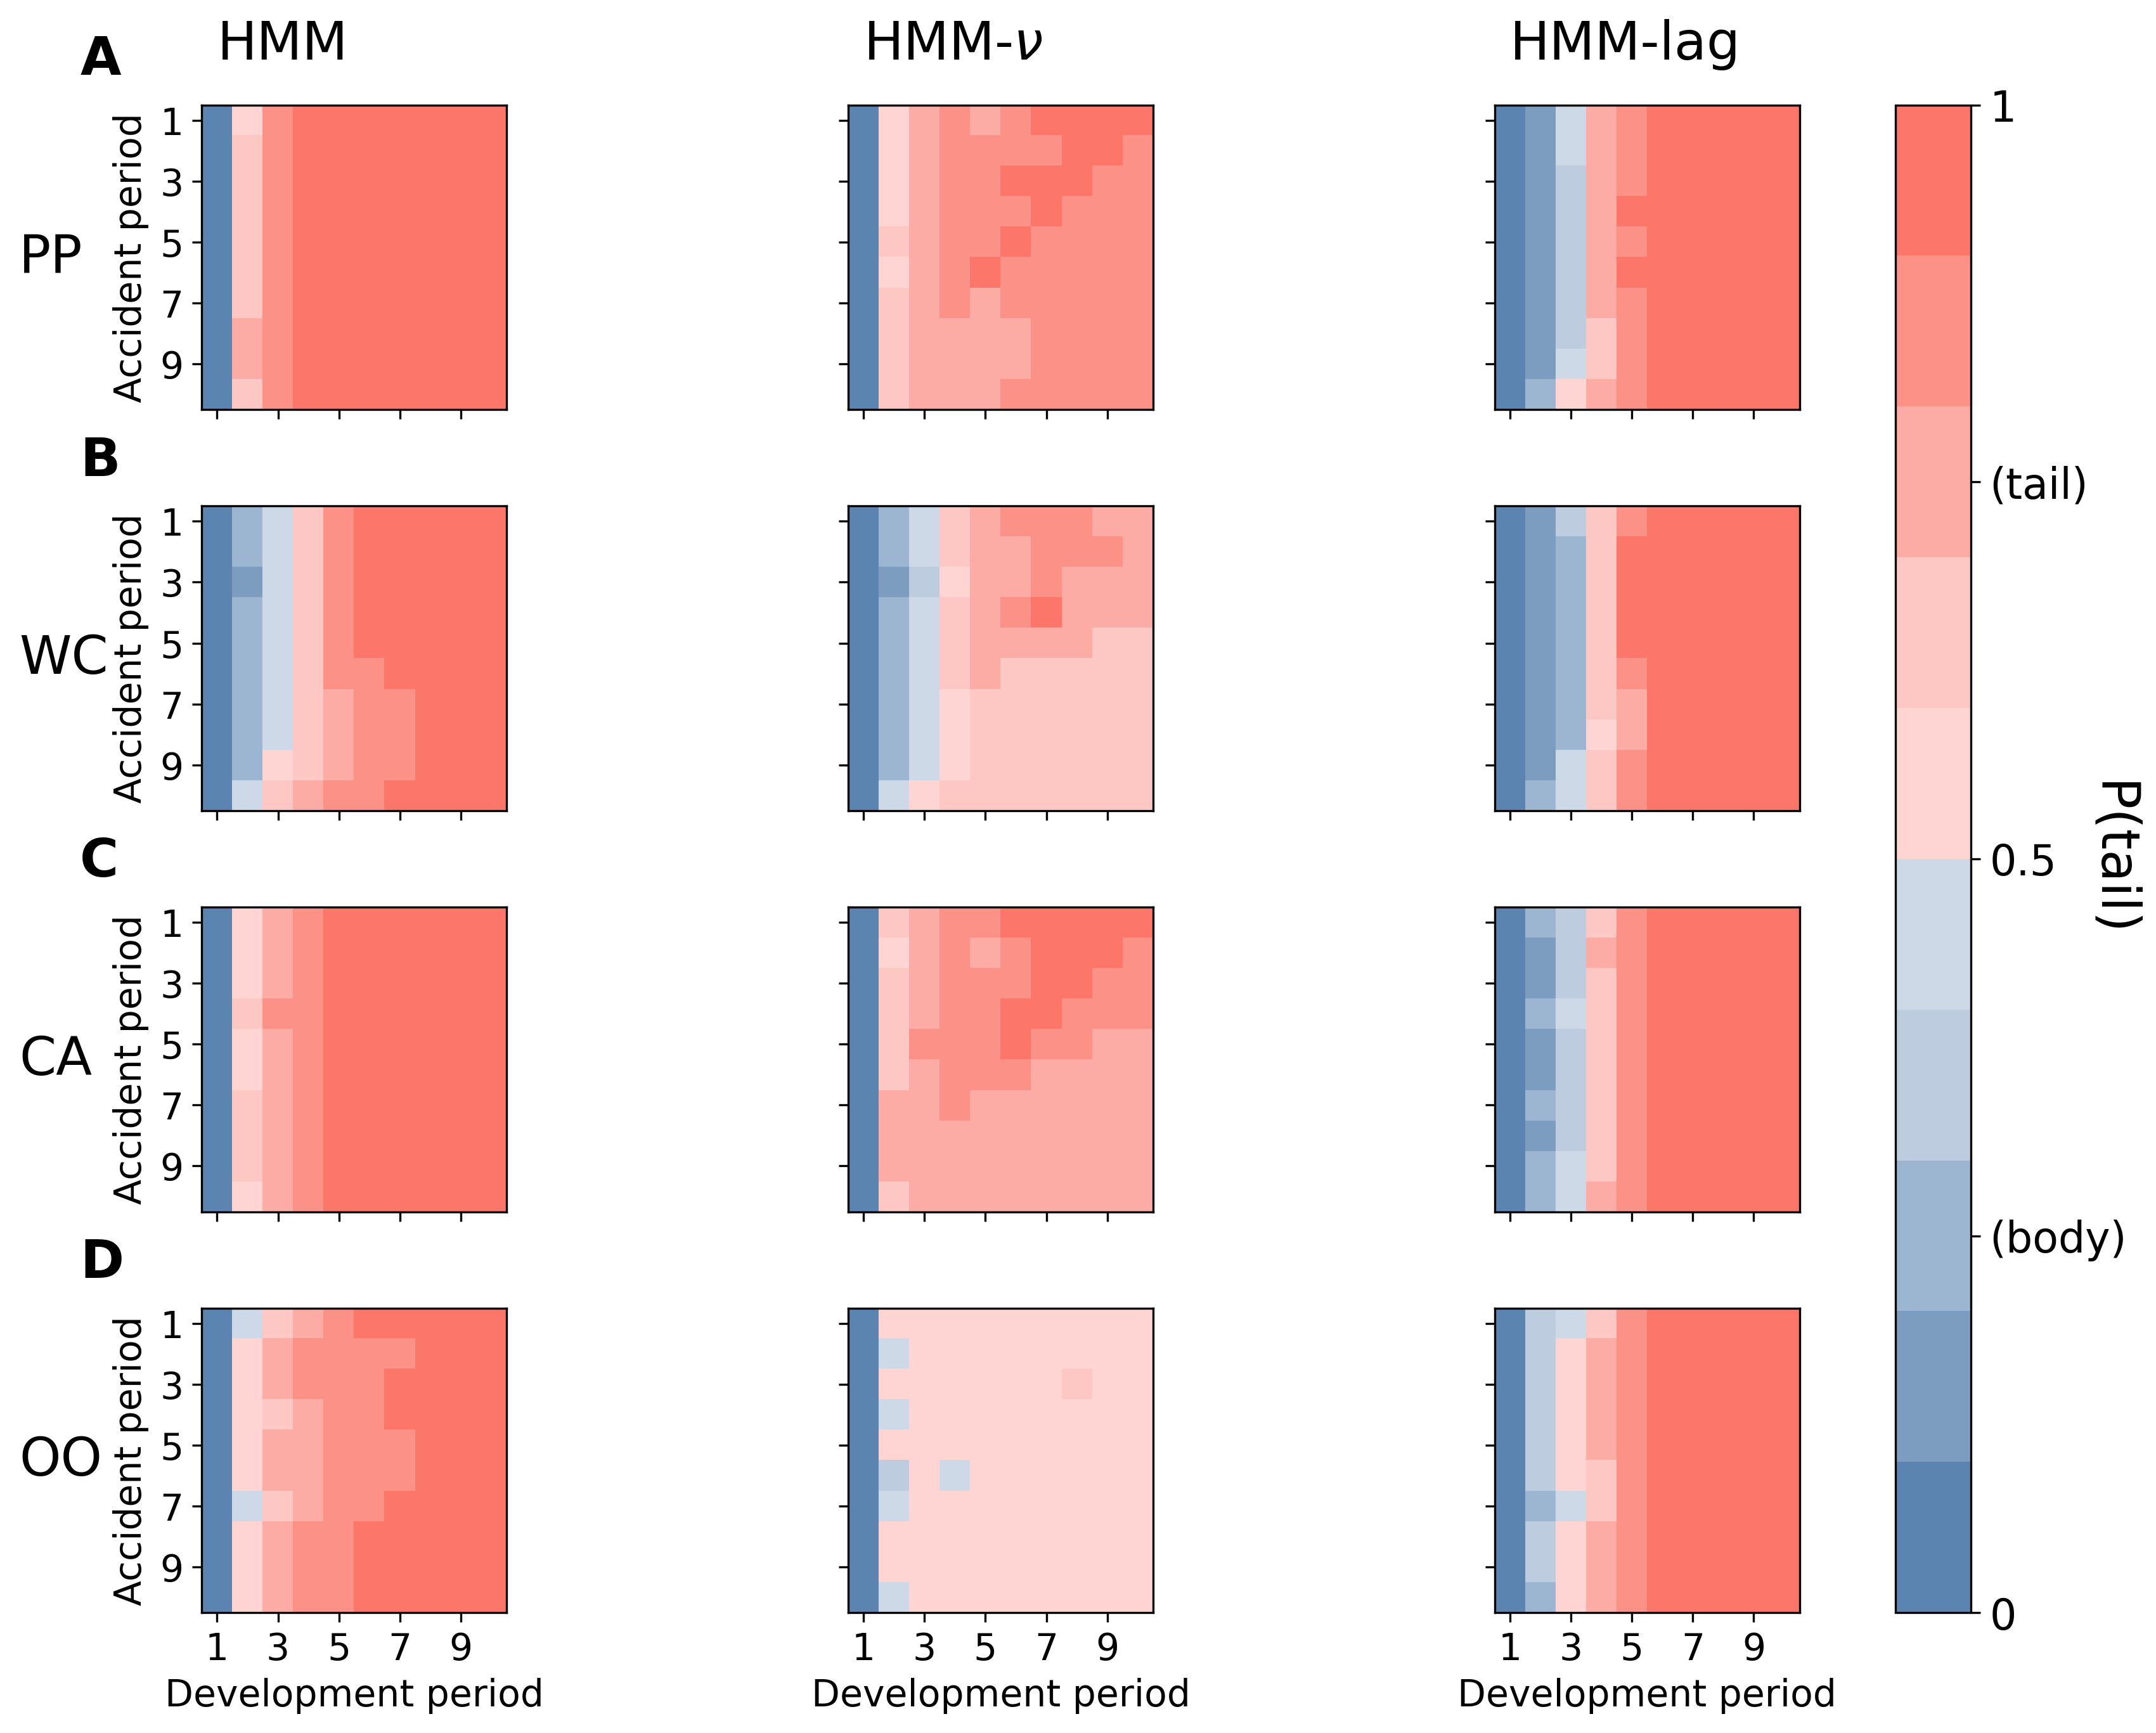
\includegraphics[scale=0.5]{\figures/z_stars.png}
    \caption{
        The average probability of being in the tail process
        for each hidden Markov model parameterization
        and line of business in the backtest data.
        Probabilities $\leq 0.5$ are coloured
        in blue whereas probabilities $> 0.5$
        are coloured in green. Faded squares
        indicating smaller probabilities of being
        in body and tail processes, respectively.
    }
\end{figure}
